\documentclass[11pt]{article}
\usepackage{graphicx, enumerate, amsmath}
\graphicspath{ {./img/} }
\parindent 0px
\date{February 2, 2024}
\title{CS362 :\hspace{2px}: Homework 1}
\author{Ryan Magdaleno}

% Helpful ::
% \line(1,0){358px}

\begin{document}
\maketitle

%%%%%%%%%%%%%%%%%%%%%%%%%%%%%%%%%%%%%%%%%%%%%%%%%%%%%%%%%%%%%%%%%%%%%%%%%%%%%%%%%%%%%%%%%

\textbf{Problem 1.} Consider the following circuits. The resistors are shown as
empty rectangles in the diagrams below.
\begin{center}
    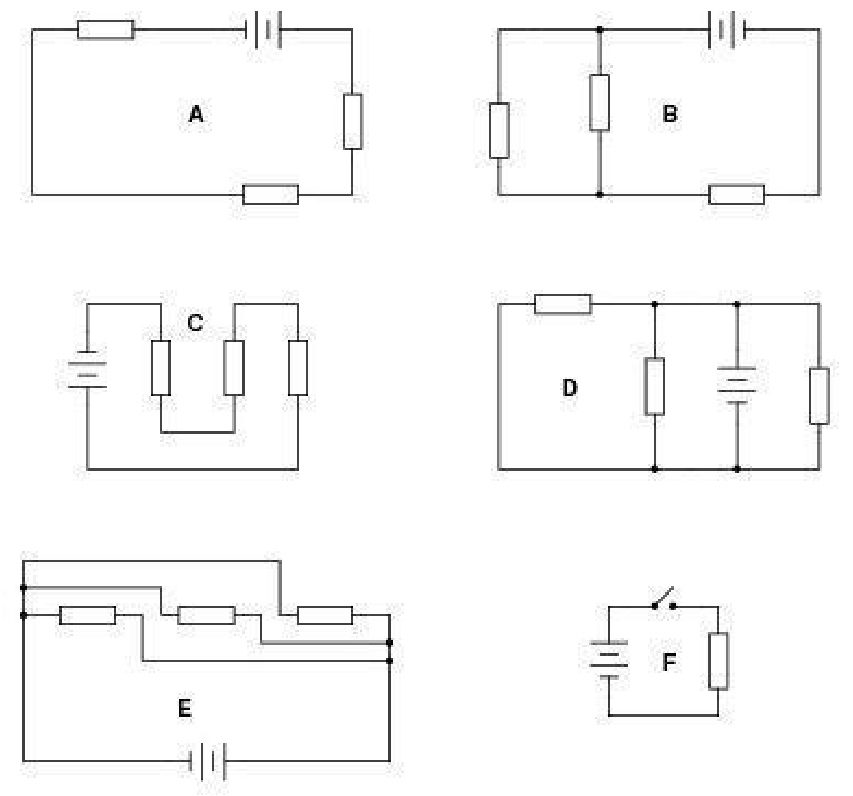
\includegraphics[scale=0.2]{1.png}
\end{center}

\vspace{5px}\textbf{Solution ::}
\begin{enumerate}[a)]
\item
Identify which of these circuits contains resistors only in series.
$$A, C, F$$

\item
Identify which of these circuits contains resistors only in parallel.
$$D, E$$

\item
Identify which of these circuit contain resistors in a combination of 
both series and parallel.
$$B$$

\end{enumerate}
\pagebreak

%%%%%%%%%%%%%%%%%%%%%%%%%%%%%%%%%%%%%%%%%%%%%%%%%%%%%%%%%%%%%%%%%%%%%%%%%%%%%%%%%%%%%%%%%

\textbf{Problem 2.} Calculate appropriate values for each of the following series circuits. Show your work.



\vspace{5px}\textbf{Solution ::}
\begin{enumerate}[a)]
\item ::
\begin{center}
    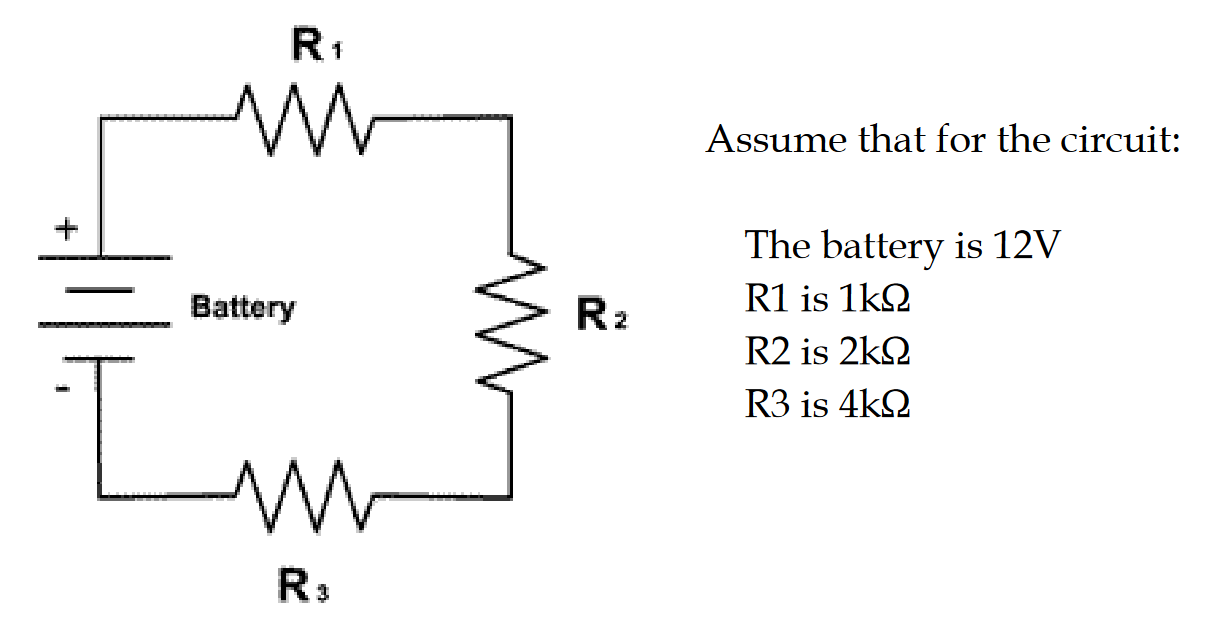
\includegraphics[scale=0.2]{2a.png}
\end{center}
Determine the total Resistance for the circuit.
\begin{align*}
    R_T&=R_1+R_2+R_3 \\
    R_T&=1\text{k}\,\Omega + 2\text{k}\,\Omega + 4\text{k}\,\Omega \\
    R_T&= 7\text{k}\,\Omega
\end{align*}
Determine the Current for the entire circuit.
\begin{align*}
    I &= \frac{V}{R_T} \\
    I &= \frac{12}{7000}
\end{align*}

Determine the Voltage Drop across each of the 3 resistors.
\begin{align*}
    V_1 = IR_1 &= \frac{12}{7000}\cdot1000 \approx 1.71429V \\
    V_2 = IR_2 &= \frac{12}{7000}\cdot2000 \approx 3.42857V \\
    V_3 = IR_2 &= \frac{12}{7000}\cdot4000 \approx 6.85714V \\
    12V &= V_1 + V_2 + V_3
\end{align*}
\pagebreak

\item ::
\begin{center}
    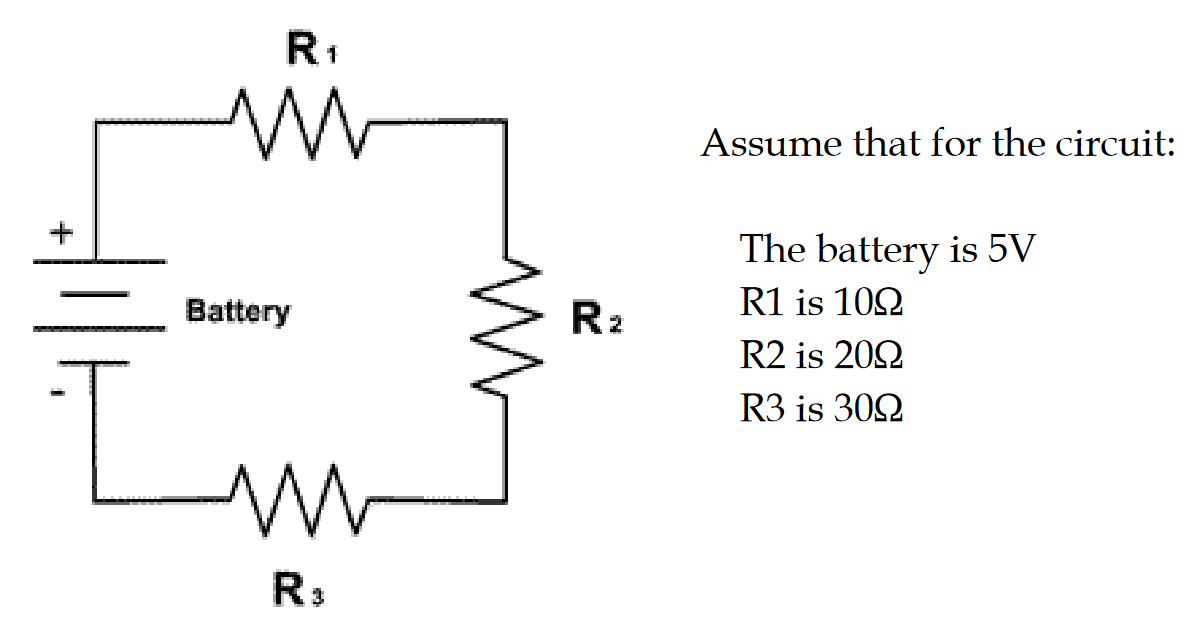
\includegraphics[scale=0.2]{2b.png}
\end{center}
Determine the total Resistance for the circuit.
\begin{align*}
    R_T&=R_1+R_2+R_3 \\
    R_T&=10\,\Omega + 20\,\Omega + 30\,\Omega \\
    R_T&= 60\,\Omega
\end{align*}

Determine the Current for the entire circuit.
\begin{align*}
    I &= \frac{V}{R_T} \\
    I &= \frac{5}{60} \\
    I &= 0.08\overline{3}A
\end{align*}

Determine the Voltage Drop across each of the 3 resistors.
\begin{align*}
    V_1 = IR_1 &= 0.08\overline{3}\cdot10 = 0.8\overline{3}V \\
    V_2 = IR_2 &= 0.08\overline{3}\cdot20 = 1.\overline{6}V \\
    V_3 = IR_2 &= 0.08\overline{3}\cdot30 = 2.5V \\
    5V &= V_1 + V_2 + V_3
\end{align*}
\end{enumerate}
\pagebreak

%%%%%%%%%%%%%%%%%%%%%%%%%%%%%%%%%%%%%%%%%%%%%%%%%%%%%%%%%%%%%%%%%%%%%%%%%%%%%%%%%%%%%%%%%

\textbf{Problem 3.} Calculate appropriate values for each of the following parallel circuits. Show your work.

\vspace{5px}\textbf{Solution ::}
\begin{enumerate}[a)]
\item ::
\begin{center}
    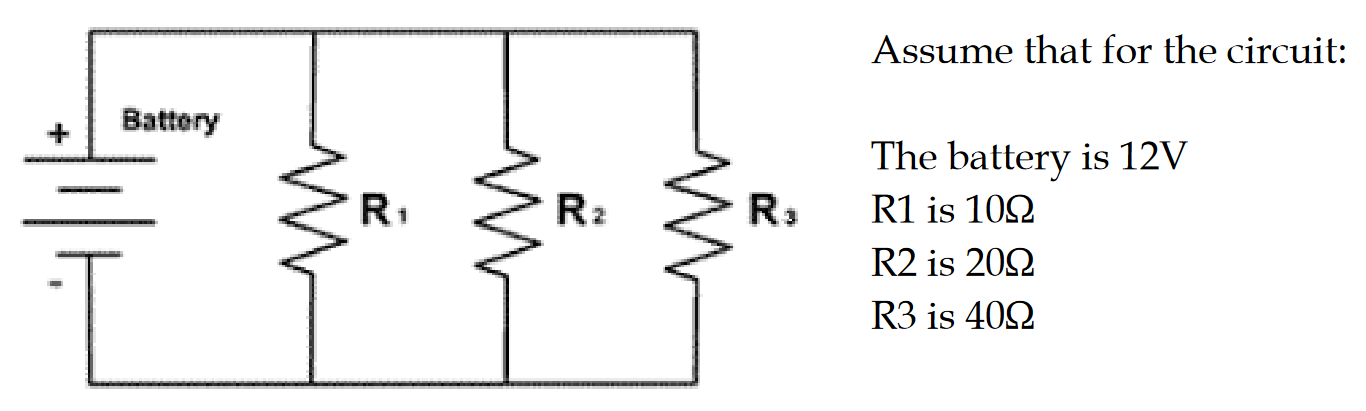
\includegraphics[scale=0.2]{3a.png}
\end{center}
Determine the total Resistance for the circuit.
\begin{align*}
    \frac{1}{R_T} &= \frac{1}{R_1} + \frac{1}{R_2} + \frac{1}{R_3} \\
    \frac{1}{R_T} &= \frac{1}{10} + \frac{1}{20} + \frac{1}{40} \\
    \frac{1}{R_T} &= 0.175\,\Omega \\
    R_T &= \frac{40}{7} \approx 5.71429\,\Omega
\end{align*}

Determine the Current for the entire circuit.
\begin{align*}
    I_{in} &= \frac{V}{R_T} \\
    I_{in} &= \frac{12}{\frac{40}{7}} \\
    I_{in} &= 2.1A
\end{align*}

Determine the Current passing through each of the 3 resistors.
\begin{align*}
    I_i &= \left(\frac{R_T}{R_i}\right)\cdot I_{in} \\
    I_1 &= \left(\frac{\approx5.71429}{10}\right)\cdot 2.1 = 1.2A \\
    I_2 &= \left(\frac{\approx5.71429}{20}\right)\cdot 2.1 = 0.6A \\
    I_3 &= \left(\frac{\approx5.71429}{40}\right)\cdot 2.1 = 0.3A
\end{align*}

\pagebreak
\item ::
\begin{center}
    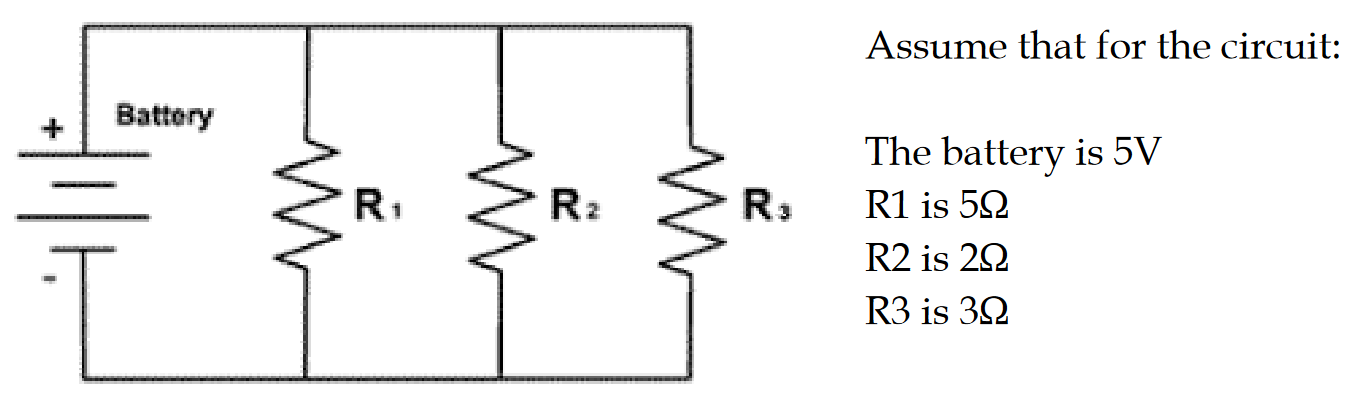
\includegraphics[scale=0.2]{3b.png}
\end{center}
Determine the total Resistance for the circuit.
\begin{align*}
    \frac{1}{R_T} &= \frac{1}{R_1} + \frac{1}{R_2} + \frac{1}{R_3} \\
    \frac{1}{R_T} &= \frac{1}{5} + \frac{1}{2} + \frac{1}{3} \\
    \frac{1}{R_T} &= 1.0\overline{3}\,\Omega \\
    R_T &= \frac{30}{31} \approx 0.96774\,\Omega
\end{align*}

Determine the Current for the entire circuit.
\begin{align*}
    I_{in} &= \frac{V}{R_T} \\
    I_{in} &= \frac{5}{\frac{30}{31}} = \frac{31}{6}\\
    I_{in} &= 5.1\overline{6}A
\end{align*}

Determine the Current passing through each of the 3 resistors.
\begin{align*}
    I_i &= \left(\frac{R_T}{R_i}\right)\cdot I_{in} \\
    I_1 &= \left(\frac{\approx0.96774}{5}\right)\cdot 5.1\overline{6} = 1A \\
    I_2 &= \left(\frac{\approx0.96774}{2}\right)\cdot 5.1\overline{6} = 2.5A \\
    I_3 &= \left(\frac{\approx0.96774}{3}\right)\cdot 5.1\overline{6} = 1.\overline{6}A
\end{align*}

\end{enumerate}
\pagebreak

%%%%%%%%%%%%%%%%%%%%%%%%%%%%%%%%%%%%%%%%%%%%%%%%%%%%%%%%%%%%%%%%%%%%%%%%%%%%%%%%%%%%%%%%%

\textbf{Problem 4.} Calculate appropriate values for each of the following
circuits. Show your work.

\vspace{5px}\textbf{Solution ::}
\begin{enumerate}[a)]
\item ::
\begin{center}
    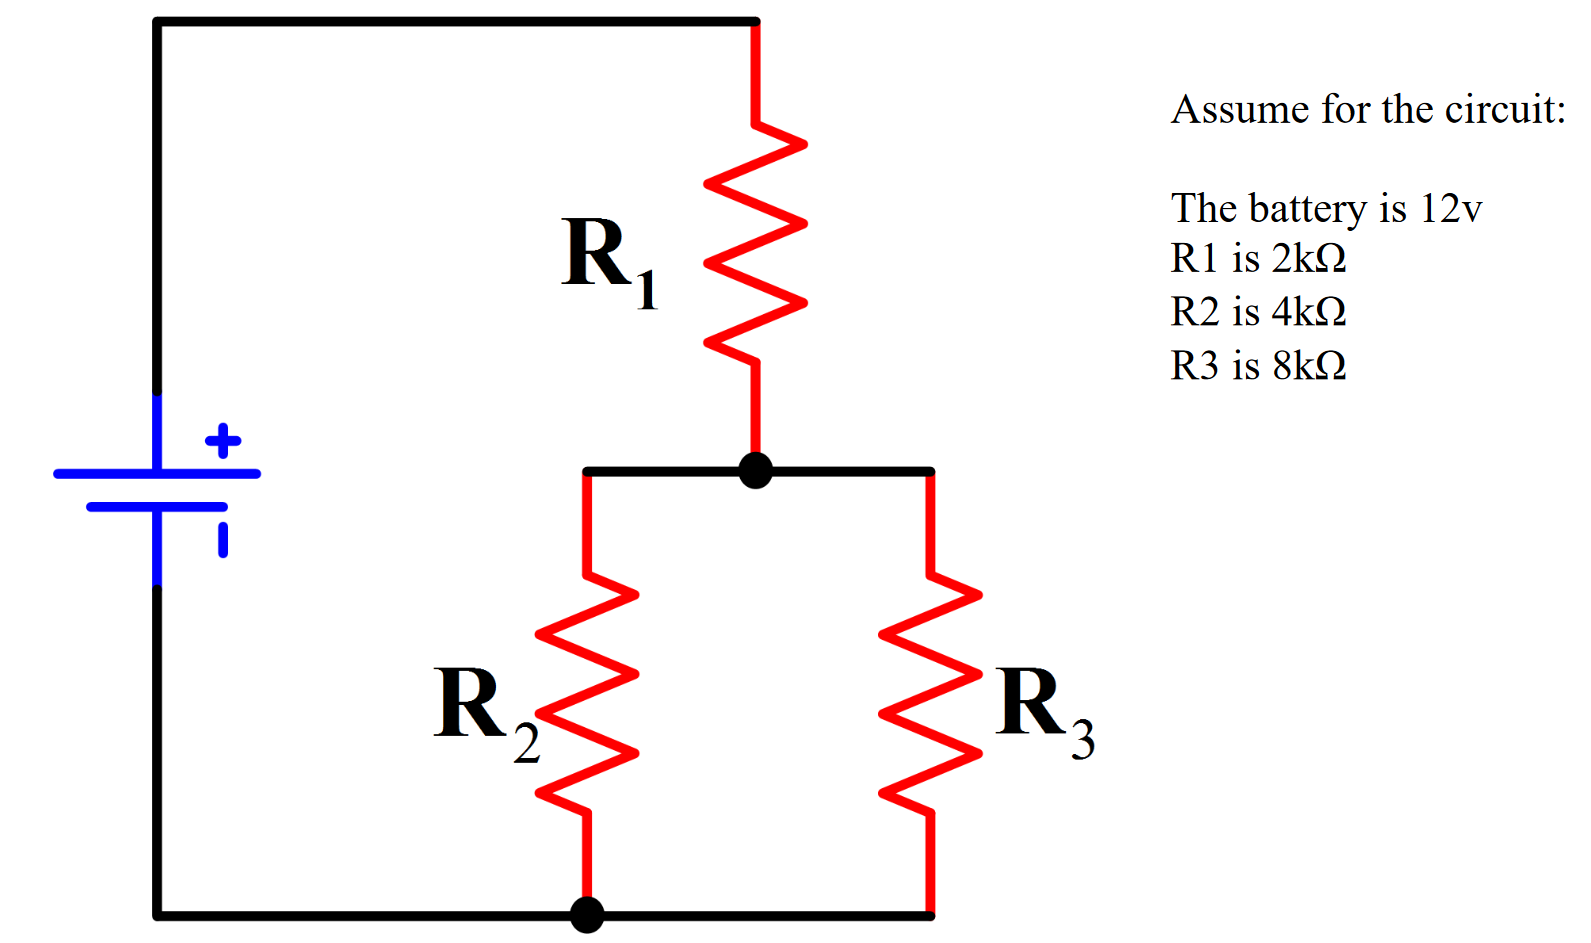
\includegraphics[scale=0.2]{4a.png}
\end{center}
Determine the total Resistance for the circuit.
\begin{align*}
    R_T &= 2000 + \frac{1}{\frac{1}{4000}+\frac{1}{8000}} \\
    R_T &= \frac{14000}{3} = 4666.\overline{6}\,\Omega
\end{align*}
Determine the Current for the entire circuit.
\begin{align*}
    I_{in} &= \frac{12}{4666.\overline{6}} \\
    I_{in} &= \frac{9}{3500} \approx 0.00257A
\end{align*}
Determine the Current passing through each of the 3 resistors.
\begin{align*}
    I_1 &= I_{in} \approx 0.00257A \\
    I_2 &= 0.00257\cdot\left(\frac{2666.6}{4000}\right) \approx 0.00171A \\
    I_3 &= 0.00257\cdot\left(\frac{2666.6}{8000}\right) \approx 0.00086 A
\end{align*}

\pagebreak
\item ::
\begin{center}
    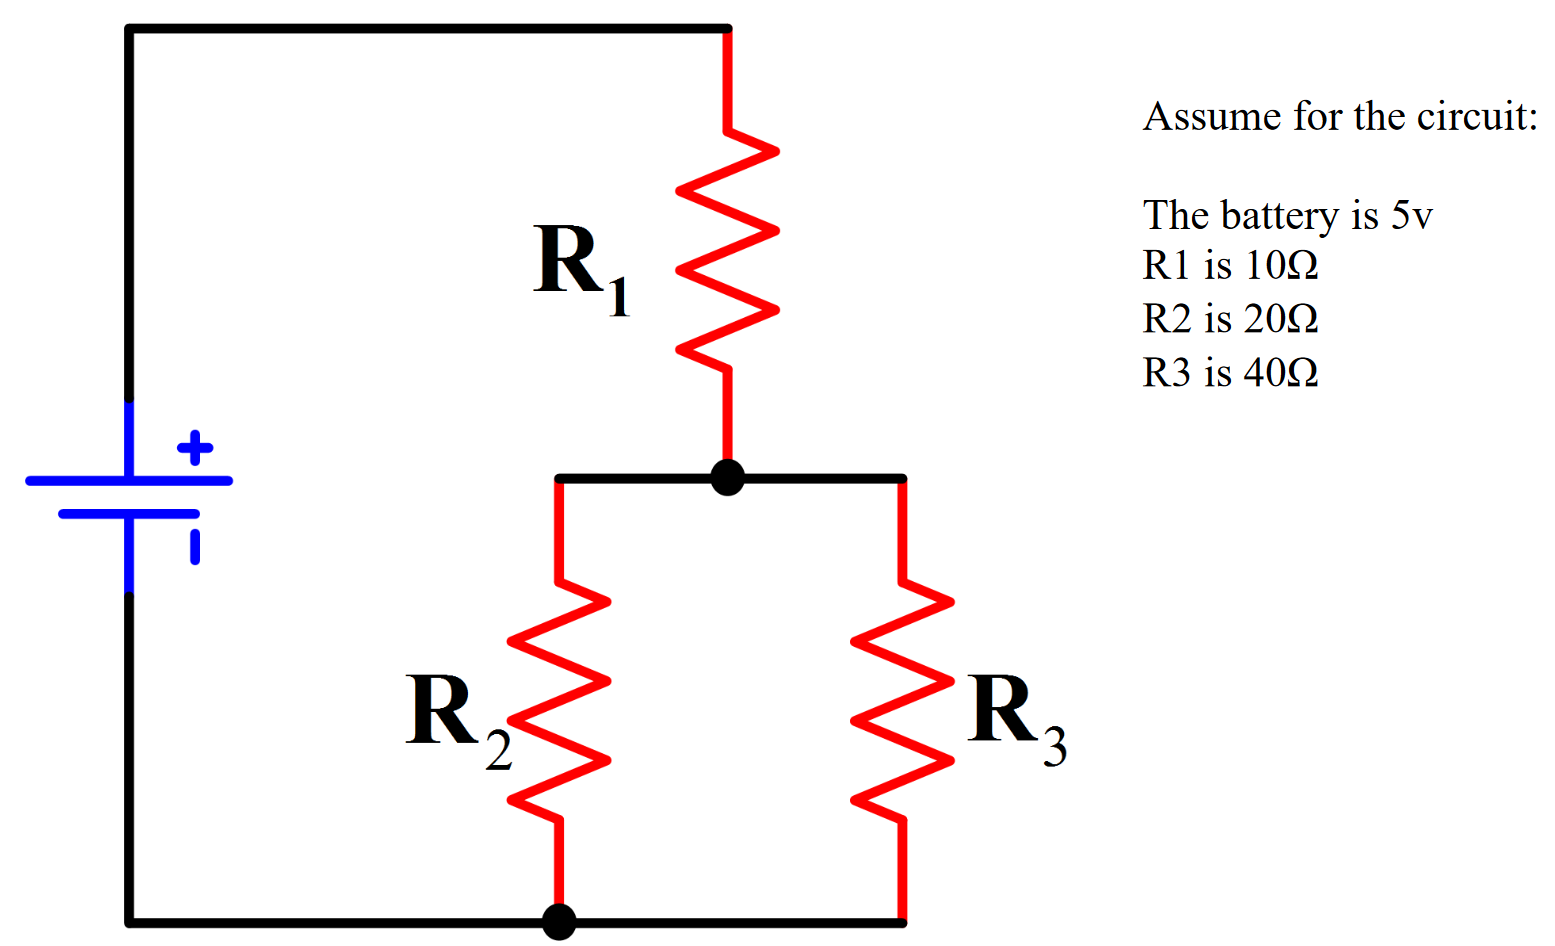
\includegraphics[scale=0.2]{4b.png}
\end{center}
Determine the total Resistance for the circuit.
\begin{align*}
    R_T &= 10 + \frac{1}{\frac{1}{20}+\frac{1}{40}} \\
    R_T &= \frac{70}{3} = 23.\overline{3}\,\Omega
\end{align*}

Determine the Current for the entire circuit.
\begin{align*}
    I_{in} &= \frac{5}{23.\overline{3}} \\
    I_{in} &= \frac{3}{14} \approx 0.21429A
\end{align*}

Determine the Current passing through each of the 3 resistors.
\begin{align*}
    I_1 &= I_{in} \approx 0.21429A \\
    I_2 &= \frac{3}{14}\cdot\left(\frac{13.\overline{3}}{20}\right)\approx0.00143A\\
    I_3 &= \frac{3}{14}\cdot\left(\frac{13.\overline{3}}{40}\right)\approx0.00071A
\end{align*}
\end{enumerate}
\pagebreak

%%%%%%%%%%%%%%%%%%%%%%%%%%%%%%%%%%%%%%%%%%%%%%%%%%%%%%%%%%%%%%%%%%%%%%%%%%%%%%%%%%%%%%%%%

\textbf{Problem 5a.} You have a circuit with a 5 volt power source, a 470 ohm
resistor, and an LED. Assume your 5V power supply stops working, but you have
a 12V power supply. You want to keep the current at the LED the same. What
resistor value would be needed if you changed your power source from 5 volts to
12 volts and, you want to keep the current at the LED the same? Assume that
the LED adds no resistance to the current.
\begin{center}
    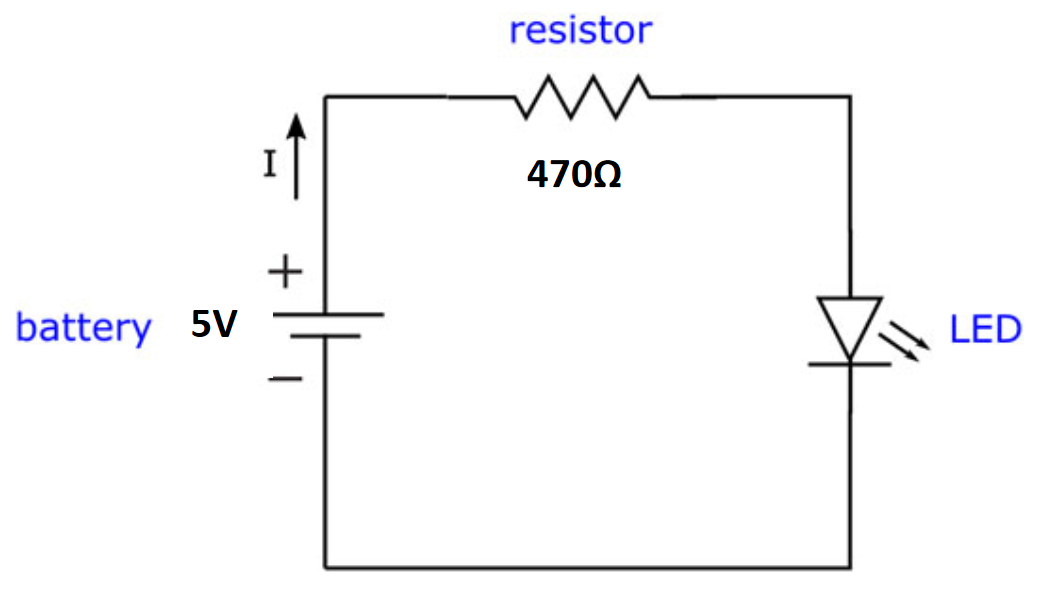
\includegraphics[scale=0.2]{5a.png}
\end{center}
\vspace{5px}\textbf{Solution ::} 
\begin{align}
    I_1 &= \frac{5}{470} = \frac{1}{94} \approx 0.01064A \\
    R_1 &= \frac{V}{I_1}\\
    R_1 &= \frac{12}{\frac{1}{94}} \\
    R_1 &= 1128\,\Omega
\end{align}


\pagebreak

%%%%%%%%%%%%%%%%%%%%%%%%%%%%%%%%%%%%%%%%%%%%%%%%%%%%%%%%%%%%%%%%%%%%%%%%%%%%%%%%%%%%%%%%%

\textbf{Problem 5b.} You have a circuit with a 5 volt power source, a 470 ohm
resistor, and an LED. However, assume the LED adds a resistance value of 80
ohms to the circuit. As with the previous problem, your 5V power supply stops
working, but you have a 12V power supply. You want to keep the current at the
LED the same. What resistor value would be needed if you changed your power
source from 5 volts to 12 volts and, you want to keep the current at the LED
the same?
\begin{center}
    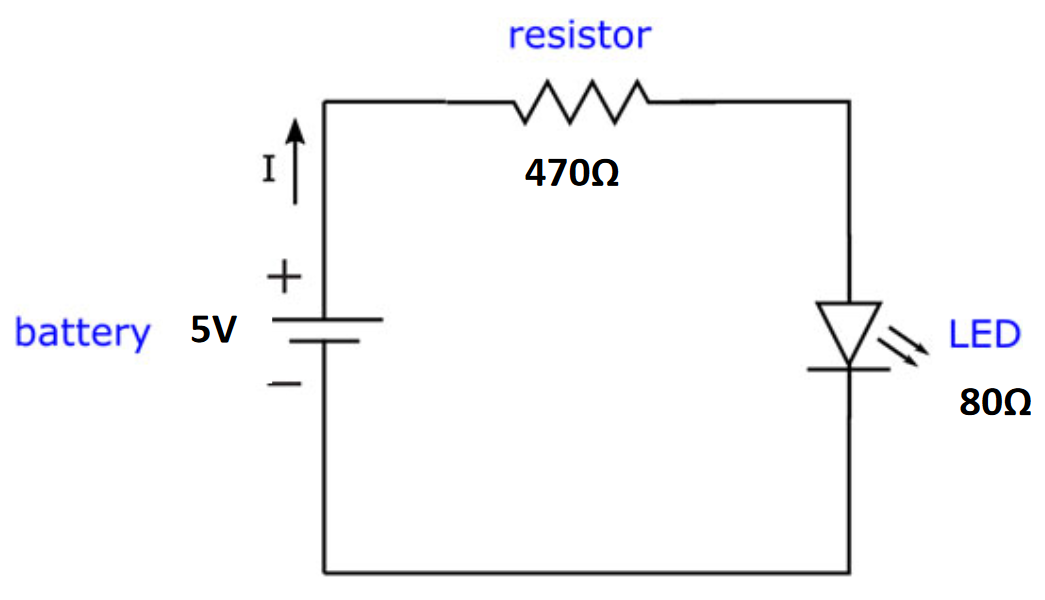
\includegraphics[scale=0.2]{5b.png}
\end{center}
\vspace{5px}\textbf{Solution ::}
\begin{align}
    R_T &= 470 + 80 = 550\,\Omega \\
    I &= \frac{V}{R_T} = \frac{5}{550} = 0.009\overline{09}A \\
    &\text{12V change but same current.} \\
    R_T &= \frac{12}{0.009\overline{09}} = 1320\,\Omega \\
    R_{1} &= R_{T} - R_{LED} \\
    R_{1} &= 1320 - 80 \\
    R_{1} &= 1240\,\Omega
\end{align}
\end{document}